%%%%%%%%%%%%%%%%%%%%%%%%%%%%%%%%%%%%%%%%%%%%%%%%%%%%%%%%%%%%%%%%%%%%
%%%%%%%%%%%%%%%%%%%%%%%%%%%%%%%%%%%%%%%%%%%%%%%%%%%%%%%%%%%%%%%%%%%%
%%                                                                %%
%% Esimerkki opinnäytteen tekemisestä LaTeX:lla 20130926          %%
%% Alkuperäinen versio Luis Costa,  muutokset Perttu Puska        %%
%%                                                                %%
%% Tähän esimerkkiin kuuluu tiedostot                             %%
%%               opinnaytepohja.tex (versio 1.7)                  %%
%%               aaltothesis.sty (versio 1.7)                     %%
%%               kuva1.eps                                        %%
%%               kuva2.eps                                        %%
%%                                                                %%
%%                                                                %%
%% Kääntäminen                                                    %%
%% latex:                                                         %%
%%             $ latex opinnaytepohja                             %%
%%             $ latex opinnaytepohja                             %%
%%                                                                %%
%%   Tuloksena on tiedosto opinnayte.dvi, joka                    %%
%%   muutetaan ps-muotoon seuraavasti                             %%
%%                                                                %%
%%             $ dvips opinnaytepohja -o                          %%
%%                                                                %%
%% Selittävät kommentit on tässä esimerkissä varustettu           %%
%% %%-merkeillä ja muutokset, joita käyttäjä voi tehdä,           %%
%% on varustettu %-merkeillä                                      %%
%%                                                                %%
%%%%%%%%%%%%%%%%%%%%%%%%%%%%%%%%%%%%%%%%%%%%%%%%%%%%%%%%%%%%%%%%%%%%
%%%%%%%%%%%%%%%%%%%%%%%%%%%%%%%%%%%%%%%%%%%%%%%%%%%%%%%%%%%%%%%%%%%%

%% Käytä toinen näistä, jos kirjoitat suomeksi:
%% ensimmäinen, jos käytät pdflatexia (kuvat on oltava pdf-tiedostoina)
%% toinen, jos haluat tuottaa ps-tiedostoa (käytä eps-formaattia kuville).
%%
%% Use one of these you write in Finnish:
%% the 1st when using pdflatex (use pdf figures) or
%% the 2nd when producing a ps file (use eps figures).
\documentclass[finnish,12pt,a4paper,pdftex]{article}
%\documentclass[finnish,12pt,a4paper,dvips]{article}


%% Käytä näitä, jos kirjoitat englanniksi
%%
%% Uncomment one of these if you write in English
%\documentclass[english,12pt,a4paper,pdftex]{article}
%\documentclass[english,12pt,a4paper,dvips]{article}

%% Tämä paketti on pakollinen
%% Valitse korkeakoulusi näistä: arts, biz, chem, elec, eng, sci.
%% Valiste editorisi käyttämä merkkikoodaustapa: utf8, latin1
%%
%% This package is required
%% Choose your school from arts, biz, chem, elec, eng, sci.
%% Choose the character encoding scheme used by your editor: utf8, latin1
\usepackage[sci,utf8]{aaltothesis} % this is the default in aaltothesis.sty
%\usepackage[elec,latin1]{aaltothesis}

%% Jos käytät latex-komentoa käännettäessä (oletusarvo), 
%% kuvat kannattaa tehdä eps-muotoon. Älä käytä ps-muotoisia kuvia!
%% Käytä seuraavaa latex-komennon ja eps-kuvien kanssa 
%%
%% Jos taas käytät pdflatex-komentoa, joka kääntää tekstin suoraan
%% pdf-tiedostoksi, kuvasi on oltava jpg-formaatissa tai pdf-formaatissa.
%%
%% Use this if you run pdflatex and use jpg/pdf-format pictures.
%%
\usepackage{graphicx}

%% Jos et jostain syystä pidä, miten alla oleva hyperref-paketti käyttää
%% fontteja, värejä yms., käytä tämän paketin makroja muuttamaan
%% fonttimäärittelyt. Katso paketin dokumentaatiota. Paketti määrittelee
%% \url-makron, joten ota paketti käyttöön, jos et käytä hyperref-pakettia.
%%
%% Use the macros in this package to change how the hyperref package below 
%% typesets its hypertext -- hyperlink colour, font, etc. See the package
%% documentation. It also defines the \url macro, so use the package when 
%% not using the hyperref package.
%\usepackage{url}

%% Saat pdf-tiedoston viittaukset ja linkit kuntoon seuraavalla paketilla.
%% Paketti toimii erityisen hyvin pdflatexin kanssa. 
%%
%% Use this if you want to get links and nice output with pdflatex
%%
\usepackage[pdfpagemode=None,colorlinks=true,urlcolor=red,%
linkcolor=blue,citecolor=black,pdfstartview=FitH]{hyperref}

\usepackage[round]{natbib}
\bibliographystyle{agsm}

%% Matematiikan fontteja, symboleja ja muotoiluja lisää, näitä tarvitaan usein 
%%
%% Use this if you write hard core mathematics, these are usually needed
\usepackage{amsfonts,amssymb,amsbsy}  

%% Vaakasuunnan mitat, ÄLÄ KOSKE!
\setlength{\hoffset}{-1in}
\setlength{\oddsidemargin}{35mm}
\setlength{\evensidemargin}{25mm}
\setlength{\textwidth}{15cm}
%% Pystysuunnan mitat, ÄLÄ KOSKE!
\setlength{\voffset}{-1in}
\setlength{\headsep}{7mm}
\setlength{\headheight}{1em}
\setlength{\topmargin}{25mm-\headheight-\headsep}
\setlength{\textheight}{23cm}


%% Kaikki mikä paperille tulostuu, on tämän jälkeen
%%
%% Output starts here
\begin{document}

%% Korjaa vastaamaan korkeakouluasi, jos automaattisesti asetettu nimi on 
%% virheellinen 
%%
%% Change the school field to describe your school if the autimatically 
%% set name is wrong
% \university{aalto University}{aalto-Yliopisto}
% \school{School of Science}{Perustieteiden korkeakoulu}

%% Vain kandityölle: Korjaa seuraavat vastaamaan koulutusohjelmaasi
%%
%% Only for B.Sc. thesis: Choose your degree programme. 
%%\degreeprogram{Electronics and electrical engineering}%
%%{Elektroniikka ja sähkötekniikka}
%%

%% Vain DI/M.Sc.- ja lisensiaatintyölle: valitse laitos, 
%% professuuri ja sen professuurikoodi. 
%%
%% Only for M.Sc. and Licentiate thesis: Choose your department,
%% professorship and professorship code. 
%%\department{Department of Radio Science and Technology}%
%%{Radiotieteen ja -tekniikan laitos}
\professorship{ICT Business}{ICT liiketoiminta}
\code{???}
%%

%% Valitse yksi näistä kolmesta
%%
%% Choose one of these:
%\univdegree{BSc}
\univdegree{MSc}
%\univdegree{Lic}

%% Oma nimi
%%
%% Should be self explanatory...
\author{Jaakko Lehtinen}

%% Opinnäytteen otsikko tulee vain tähän. Älä tavuta otsikkoa ja
%% vältä liian pitkää otsikkotekstiä. Jos latex ryhmittelee otsikon
%% huonosti, voit joutua pakottamaan rivinvaihdon \\ kontrollimerkillä.
%% Muista että otsikkoja ei tavuteta! 
%% Jos otsikossa on ja-sana, se ei jää rivin viimeiseksi sanaksi 
%% vaan aloittaa uuden rivin.
%% 
%% Your thesis title. If the title is very long and the latex 
%% does unsatisfactory job of breaking the lines, you will have to
%% break the lines yourself with \\ control character. 
%% Do not hyphenate titles.
\thesistitle{Thesis template}{LISÄÄ NIMI}

\place{Espoo}
%% Kandidaatintyön päivämäärä on sen esityspäivämäärä! 
%% 
%% For B.Sc. thesis use the date when you present your thesis. 
\date{KORJAA: 24.9.2013}

%% Kandidaattiseminaarin vastuuopettaja tai diplomityön valvoja.
%% Huomaa tittelissä "\" -merkki pisteen jälkeen, 
%% ennen välilyöntiä ja seuraavaa merkkijonoa. 
%% Näin tehdään, koska kyseessä ei ole lauseen loppu, jonka jälkeen tulee 
%% hieman pidempi väli vaan halutaan tavallinen väli.
%%
%% B.Sc. or M.Sc. thesis supervisor 
%% Note the "\" after the comma. This forces the following space to be 
%% a normal interword space, not the space that starts a new sentence. 
\supervisor{Prof.\ Martti Mäntylä}{Prof.\ Martti Mäntylä}

%% Kandidaatintyön ohjaaja(t) tai diplomityön ohjaaja(t)
%% 
%% B.Sc. or M.Sc. thesis advisors(s). 
%%
%% Note that there has been a change in the official EN translation
%% of the Finnish title ``ohjaaja'' which in the previous version (1.5) 
%% of this document was called ``instructor''. The recommended
%% translation is now ``advisor''.  
%% However, the LaTeX internal variable remains \instructor
%% as there is little point to change the variable name. 
%%
%\instructor{Prof. Pirjo Professori}{Prof. Pirjo Professori}
%\instructor{D.Sc.\ (Tech.) Olli Ohjaaja}{TkT Olli Ohjaaja}
\instructor{M.Sc.\ (Tech.) Tapio Jakola}{DI Tapio Jakola}

%% Aaltologo: syntaksi:
%% \uselogo{aaltoRed|aaltoBlue|aaltoYellow|aaltoGray|aaltoGrayScale}{?|!|''}
%% Logon kieli on sama kuin dokumentin kieli
%%
%% Aalto logo: syntax:
% \uselogo{aaltoRed|aaltoBlue|aaltoYellow|aaltoGray|aaltoGrayScale}{?|!|''}
%% Logo language is set to be the same as the document language.
\uselogo{aaltoRed}{''}

%% Tehdään kansilehti
%%
%% Create the coverpage
\makecoverpage


%% Suomenkielinen tiivistelmä
%% 
%% Finnish abstract
%%
%% Tiivistelmän avainsanat
\keywords{Avainsanoiksi valitaan kirjoituksen sisältöä keskeisesti kuvaavia
käsitteitä}
%% Tiivistelmän tekstiosa
\begin{abstractpage}[finnish]
  Tiivistelmässä on lyhyt selvitys (noin 100 sanaa)
  kirjoituksen tärkeimmästä sisällöstä: mitä ja miten on tutkittu,
  sekä mitä tuloksia on saatu. 
  Tiivistelmässä on lyhyt selvitys (noin 100 sanaa)
  kirjoituksen tärkeimmästä sisällöstä: mitä ja miten on tutkittu,
  sekä mitä tuloksia on saatu. 

  Tiivistelmässä on lyhyt selvitys (noin 100 sanaa)
  kirjoituksen tärkeimmästä sisällöstä: mitä ja miten on tutkittu,
  sekä mitä tuloksia on saatu. 
  Tiivistelmässä on lyhyt selvitys (noin 100 sanaa)
  kirjoituksen tärkeimmästä sisällöstä: mitä ja miten on tutkittu,
  sekä mitä tuloksia on saatu. 
  Tiivistelmässä on lyhyt selvitys (noin 100 sanaa)
  kirjoituksen tärkeimmästä sisällöstä: mitä ja miten on tutkittu,
  sekä mitä tuloksia on saatu. 
\end{abstractpage}

%% Pakotetaan uusi sivu varmuuden vuoksi, jotta 
%% mahdollinen suomenkielinen ja englanninkielinen tiivistelmä
%% eivät tule vahingossakaan samalle sivulle
%%
%% Force new page so that English abstract starts from a new page
\newpage
%
%% English abstract, uncomment if you need one. 
%% 
%% Abstract keywords
\keywords{}
%% Abstract text
\begin{abstractpage}[english]
 Your abstract in English. Try to keep the abstract short, approximately 
 100 words should be enough. Abstract explains your research topic, 
 the methods you have used, and the results you obtained.  
\end{abstractpage}
%% Note that 
%% if you are writting your master's thesis in English place the English
%% abstract first followed by the possible Finnish abstract

%% Esipuhe 
%%
%% Preface
\mysection{Esipuhe}
%\mysection{Preface}
Lisää tähän esipuhe.\\

\vspace{5cm}
Otaniemi, 24.9.2013

\vspace{5mm}
{\hfill T T.\ A.\ Teekkari \hspace{1cm}}

%% Pakotetaan varmuuden vuoksi esipuheen jälkeinen osa
%% alkamaan uudelta sivulta
%%
%% Force new page after preface
\newpage


%% Sisällysluettelo
%% 
%% Table of contents. 
\thesistableofcontents


%% Symbolit ja lyhenteet
%%
%% Symbols and abbreviations
\mysection{Käsitteet}
%\mysection{Symbols and abbreviations}




%% Sivulaskurin viilausta opinnäytteen vaatimusten mukaan:
%% Aloitetaan sivunumerointi arabialaisilla numeroilla (ja jätetään
%% leipätekstin ensimmäinen sivu tyhjäksi, 
%% ks. alla \thispagestyle{empty}).
%% Pakotetaan lisäksi ensimmäinen varsinainen tekstisivu alkamaan 
%% uudelta sivulta clearpage-komennolla. 
%% clearpage on melkein samanlainen kuin newpage, mutta 
%% flushaa myös LaTeX:n floatit 
%% 
%% Corrects the page numbering, there is no need to change these
\cleardoublepage
\storeinipagenumber
\pagenumbering{arabic}
\setcounter{page}{1}


%% Leipäteksti alkaa
%%
%% Text body begins. Note that since the text body
%% is mostly in Finnish the majority of comments are
%% also in Finnish after this point. There is no point in explaining
%% Finnish-language specific thesis conventions in English.
\section{Johdanto}
%\section{Introduction}

%% Ensimmäinen sivu tyhjäksi
%% 
%% Leave first page empty
\thispagestyle{empty}

(Tarvitsee vielä paljon hiomista ja rikastamista muista lähteistä.)

Yrityksen tulee etsiä tapoja säästää resursseja ja mahdollistaa itsepalvelu sen asiakkaille kellonajasta riippumatta, ja nämä tavoitteet ovat parhaiten saavutettavissa IT-palvelujen ja prosessessien automatisoinnilla \citep{lamoureux}. Yritykset aloittivat mekaanisen automatisoinnin jo 1950-luvulla, ja jokainen teknologinen kehitysaskel sen jälkeen on mahdollistanut yhä monimutkaisempien toimintojen automatisoinnin yrityksen toiminnassa. 

Automaatio käsitteenä sai merkityksensä autoteollisuuden tuotantolinjoilta, ja tietotekniikan yleistymisen jälkeen 1970-ja 1980-luvulla yritykset oppivat hyödyntämään automaatiota myös sisäisissä, laskentaa vaativissa prosesseissa, kuten taloushallinnossa. Internetin yleistymisen myötä 1990-2000-luvuilla teknologian kehitys on mahdollistanut liiketoimintaprosessien automatisoinnin. Koko tilaus- ja toimitusketju ja useat tuotteet ja palvelut muuttuivat digitaalisiksi. Automaatiossa ei ole siis pelkästään kysymys ihmistyön antamisesta tietokoneelle, vaan myös sen tekemisestä mikä ei aikaisemmin ollut mahdollista \citep{groover}.

Digitalisaatiosta on puhuttu jo vuosia, ja toistaiseksi se on tarkoittanut sosiaalista mediaa, mobilisaatiota, big data-analytiikkaa ja pilviteknologioiden kehitystä. Digitalisaation seuraavassa vaiheessa on kysymys ohjelmistorobotiikan ja älykkään automaation hyödyntämisestä liiketoiminnan prosesseissa. Voidaan ajatella, että seuraavan ajanjakson aikana teknologia saa aisteja, jotka olivat aikaisemmin vain ihmisen yksinoikeus \citep{groover}.

Teknologisten kehitysaskelten myötä itse teknologia muuttuu kompleksimmaksi ymmärtää, mutta niiden sovelluskohteet monipuolistuvat. Yritysten välisessä kilpailussa kyky hyödyntää uutta teknologiaa ketterästi avaa pienillekin toimijoille ovet kilpailussa jättejä vastaan. Hyvä esimerkki tästä on verkkokaupan kasvu kymmenen viime vuoden aikana. Kuluttajat ovat tottuneet saamaan haluamansa palvelut käyttöönsä yhdellä painalluksella. Sama ilmiö leviää yritysten liiketoimintaan. Odotetaan yhä isompien ja monimutkaisempien palveluiden olevan mahdollisia ottaa käyttöön hetkessä. Tämä tarjoaa pienemmille toimijoille mahdollisuuksia disruptioida markkinoita yksinkertaisella kustannustehokkaalla lähestymistavalla. Teknologinen kehitys tuo yhä monipuolisempia mahdollisuuksia kenelle tahansa luoda jotain joka ei aikaisemmin ollut mahdollista. \citep{lamoureux}

Suuryrityksillä onkin yhä enemmän paineita automatisoida prosessejaan ja investoitava uuteen teknologiaan. Puhutaan transformaatiosta, jossa olemassaolevia tietojärjestelmien määrää vähennetään, toimintoja yksinkertaistetaan,  legacy-järjestelmistä yritetään päästä eroon ja pyritään muuttamaan toimintamalli ketteräksi. Onneksi uudet teknologiat mahdollistavat tämän. Ei ole tarvetta yrittää toimia kuin start up-yritys, on tärkeämpää ymmärtää yritykselle relevantteja teknologioita ja niiden liiketoimintahyötyjä omassa kontekstissa. \citep{lamoureux}

Operaattorin näkökulmasta ilmassa on mahdollisuuksia ja uhkia. McKinseyn tekemän raportin mukaan operaattorit ovat suuressa vaarassa kärsiä disruptiosta markkinoilla. Viiden viime vuoden aikana liikevaihto alalla on ollut hitaasti laskemassa kovan hintakilpailun vuoksi, ja silti investointeja on tehtävä. Data vie koko ajan tilaa perinteisiltä tuottavilta puhe- ja viestintäpalveluilta. Operaattorit ovat vaarassa jäädä tietoliikenneyhteyksien toimittajan rooliin. Onneksi mahdollisuudetkin ovat suuret liiketoiminnan prosessien ja tarjoomien uudistuessa. Raportin mukaan yksi mahdollisuus on kehittää palveluita strategisten kumppaneiden kanssa tavalla, jossa tuotannon ja toimituksen kustannukset ovat minimoitu automatisoinnilla ja digitaalisen asiakaskokemuksen luomisella itsepalvelukanavien kautta.\citep{mckinseytele}

(Tähän parempi aasinsilta)

Asiakaspalveluratkaisujen (contact center) tarjoaminen yritysasiakkaille on ollut operaattoreiden luontaista liiketoimintaa ydinliiketoiminnan ohella. Asiakaspalvelujärjestelmät tarkoittavat yrityksen asiakkaiden yhteydenottojen käsittelemistä yhden järjestelmän kautta kanavasta riippumatta. Operaattorit ovat olleet vahvoilla tässä liiketoiminnassa puhelinverkkojensa ansiosta. Teknologian kehittymisen myötä puhelinkanavan rinnalle on tullut muita sähköisiä kanavia, ja kanavien määrä kasvaa koko ajan sen mukaan miten asiakkaat haluavat asioida yrityksen kanssa. Kanavasta riippumatta asiakaspalvelujärjestelmän tulisi tarjota asiakaspalvelua tarjoavalle työntekijälle yksi näkymä asiakkaan tietoihin. Yrityksen järjestelmissä on erilaista tietoa asiakkaasta, joka olisi saatava helpoksi näkymäksi yrityksen työntekijälle. Asiakaspalvelujärjestelmä siis integroituu moneen eri järjestelmään ja kanavaan. Tarpeet eri integraatioille kasvavat koko ajan, koska yritykset haluavat tarjota hyvää asiakaskokemusta. Hyvään asiakaskokemukseen vaaditaan paljon tietoa eri järjestelmistä saatavilla helposti ymmärrettävässä muodossa. Asiakaspalvelujärjestelmien kehittäminen on kallista ohjelmistokehitystä, joten operaattorin on ollut helpompi tarjota valitun kumppanin tuotetta asiakkaille ja keskittyä ydinosaamiseensa, eli yhteyksien rakentamiseen asiakastoimituksissa, ja jättää itse järjestelmän kehitys kumppanille. 

Järjestelmiä tarjoavat myös muut kuin operaattorit, ja heidän kilpailuvalttinsa on ollut kustannustehokas tapa toimittaa järjestelmä, asiakaskokemus ja alhaisempi hinta. Itse puhelinkanavan merkityksen vähentyminen tarkoittaa operaattorin ainoan kilpailivaltin merkityksen vähenemistä. Näyttää siis siltä, että operaattorin asemaa asiakaspalvelujärjestelmä-markkinalla disruptoidaan. 

Tässä työssä keskitytään tarkastelemaan
Telia Finland Oyj:n asiakaspalvelujärjestelmää Kontakti L, jolle on asetettu tavoitteeksi automaattinen asiakasprosessi (tilauksen, toimituksen ja laskutuksen osalta), itsepalvelun lisääminen ja kustannustehokkuus. Kyseisellä tuotealueella ei ole aikaisemmin onnistuttu luomaan automaattista asiakasprosessia nykyisissä olosuhteissa. Tarvitaan siis selvitys siitä miten olosuhteiden tulisi muuttua automaattista asiakasprosessia varten.

\subsection{Tutkimuskysymys ja alakysymykset}

Pääkysymys:
\begin{itemize}
\item[--]Kysymys 1: Mitkä ovat ne olosuhteet, joissa Kontakti L- asiakaspalvelujärjestelmän asiakasprosessi voidaan automatisoida?
\item[--]Vastaus 1: Kuvaus automatisoidusta asiakasprosessista ja sen vaatimista olosuhteista.
\end{itemize}

Alakysymykset:
\begin{itemize}
\item[--]Kysymys 2: Mitkä ovat ne edellytykset joiden perusteella Kontakti L- asiakaspalvelujärjestelmä on kannattava tarjota digitaalisen itsepalvelukanavan kautta?
\item[--]Vastaus 2: Edellytykset digitaalisen itsepalvelukanavan hyödyntämiselle.
\item[--]Kysymys 3: Missä kohdin automatisoitua asiakasprosessia olisi järkevä hyödyntää robotiikkaa tai älykästä automaatiota?
\item[--]Vastaus 3: Asiakasprosessin vaiheet, joissa robotiikan tai älykkään automaation käyttö on perusteltua.

\end{itemize}
\subsection{Työn rakenne}
Taustatieto kappaleessa kerron yleisesti asiakasprosessista ja mitä sen automatisoinnilla voidaan saavuttaa. Kappaleessa tuodaan myös esille automaation tämän hetken trendejä. Kappale määrittää työn keskeisen konseptin.

Asiakaspalvelujärjestelmät-kappeleessa kuvataan tarkemmin minkälaisestä järjestelmästä on kysymys, eli kuvataan liiketoiminnan ongelma, jonka järjestelmä ratkaisee eri kokoisissa yrityksissä. Kappaleessa tuodaan myös esille minkälaisia järjestelmät ovat luonteeltaan ja minkälaisia tulevaisuuden trendejä on nähtävissä.

Digitaalinen visio-kappaleessa keskitytään antamaan kuva siitä minkälaisia haasteita digitalisaatio ja automatisaatio tuottavat operaattorille, ja miten näitä haasteita on alettu ratkaisemaan.

Yhteenvedossa tuodaan kappaleiden aiheet yhteen ja perustellaan miksi on olennaista tarkastella asiakasjärjestelmän asiakasprosessin automatisointia juuri Telialla.

\subsection{Tutkimuksen rajaus}


%% Opinnäytteessä jokainen osa alkaa uudelta sivulta, joten \clearpage
%%
%% In a thesis, every section starts a new page, hence \clearpage
\clearpage

\section{Taustatieto}


% \section{Background}
\subsection{Asiakasprosessi ja sen automatisoinnin arvo}


\subsubsection{Asiakasprosessi}



\subsubsection{Prosessien kehittäminen/automaatio (BPM)}

Prosessien kehittämisen pohjana toimivat samat visiot, toimintaperiaatteet ja strategiat jotka ohjaavat organisaatiota. Prosesseja kehitettäessä organisaation johdon tulee antaa toiminnalle selkeät tavoitteet sekä varata muutosten tekemiselle sekä käyttöönotolle riittävät resurssit. Tehdyt muutokset eivät saisi olla kertaluontoisia vaan niiden tulisi johtaa vaikutusten jatkuvaan mittaamiseen sekä kehittämiseen \citep{harmon}. 

Yleensä prosessien kehittämisellä tavoitellaan toiminnan tehostamista, palvelutason ja toiminnan laadun paranemista, kustannussäästöjen sekä ongelmatilanteiden hallinnan aikaansaamista. Käytännössä tämä tarkoittaa päällekkäisten työvaiheiden poistamista, asioiden uudenlaista keskittämistä tai rinnakkaisvaiheiden lisäämistä, jotta läpimenoaikaa saadaan nopeutettua. Usein tavoitteena on myös parantaa prosessin luotettavuutta ja käytettävyyttä, vähentää tarvetta moninkertaisille hyväksynnöille sekä lisätä prosessin mitattavuutta. Prosessien kehittäminen saattaa usein johtaa tilanteeseen jossa joudutaan muodostamaan uusia työtiimejä tai organisoimaan prosessit uudella tavalla. \citep{harmon}

Prosessin design viittaa toimintaan, jonka tarkoituksena on parantaa merkittävästi nykyisiä prosesseja tai luoda kokonaan uusia liiketoimintaprosesseja. Prosessin design ottaa kantaa prosessin jokaiseen osaseen ja johtaa usein prosessin osien muutoksiin, kuten ihmisten määrään prosessissa ja automaation käyttöönottoon.  \citep{harmon}

Prosessiautomaatio viittaa tietokoneiden ja ohjelmistotuotteiden käyttöä ihmistyön apuna tai ihmistyön korvaajana. BPM-termiä käytetään usein kuvaamaan prosessin automatisointiin liittyviä toimenpiteitä. Sitä käytetään myös viittaamaan automatisoidun prosessin suorittamiseen ohjelmiston avulla. \citep{harmon}

\begin{itemize}
\item[--]https://www2.deloitte.com/content/dam/Deloitte/us/Documents/process-and-operations/us-sdt-process-automation.pdf
\item[--]https://www.britannica.com/technology/automation 
\item[--]\citep{lamoureux}
The technology of automation has evolved from the related field of mechanization, which had its beginnings in the Industrial Revolution. Mechanization refers to the replacement of human (or animal) power with mechanical power of some form. The driving force behind mechanization has been humankind’s propensity to create tools and mechanical devices
\item[--]\citep{harmon}.
Business Process Change
In economically bad times, when money is tight, companies seek to make their processes more efficient. In economically good times, when money is more available, companies seek to expand, to ramp up production, and to enter new markets. They improve processes to offer better products and services in hopes of attracting new customers or taking customers away from competitors.
\item[--]

\end{itemize}






\subsection{Asiakaspalvelujärjestelmät}

Asiakaspalvelujärjestelmä ovat organisaation keskitetty toiminto, jossa käsitellään usein suurta määrää asiakkaan yhteydenottoja. Perinteisesti tärkeitä toimintoja ovat sisääntulevat ja ulos lähtevät kontaktit. Sisään tuleva liikenne on usein asiakaspalvelua ja ulospäin lähtevä liikenne proaktiivista asikaspalvelua tai myyntiä. Asiakaspalvelujärjestelmään kuitenkin keskittyy myös muita kanavia kuten sähköposti, chat ja sosiaalinen media.

Asiakaspalvelujärjestelmän käyttäjää kutsutaan agentiksi. Agentti tarvitsee useissa tapauksissa edelleen fyysisen puhelimen ja työaseman, joskin useat uudet ratkaisut pyrkivät välttämään tarvetta tälle. Agenttien on pystyttävä ratkaisemaan asiakkaiden ongelma, ja siksi onkin järkevää, että agenteilla on erilaisia taitoja, joiden perusteella asiakaskontaktit ohjautuvat heille. Nykyään on myös tavallista, että organisaatioilla ei ole erikseen suurta asiakaspalveluorganisaatiota, ja yhä useampi työntekijä kuitenkin käyttää asiakaspalvelujärjestelmää agenttina. 


\subsection{Digitaalinen visio Telialla}

\citep{lamoureux}

\begin{itemize}
\item[--]Amazon-Wallmart(Disruptor-Disrupted): Wallmart mastered cost management, supply chain efficiency & merchandising. Amazon became more valuable in just 21 years from nothing! Amazon entered mature industry, and used viable digital tech to make their processes efficient & customer buying process easy. Walmart had advantage from beginning but did not embrace digitality into its processes. Can today’s established businesses leverage digital tech to be the disruptor, not the disrupted. Existing businesses that leverage their relationships  and processes and energetically apply new, viable technologies will win.
\item[--]New technologies have become more viable to enable more efficient processes and facilitation of the customer journey, like cloud technologies for computer service or RPA 
\item[--]\citep{lamoureux}
Jatkuva viitekehys digitaalisuuteen:
Digitaaliset teknologiat - liiketoiminnallinen käyttökohde - Liiketoiminnan tulos
\item[--]\citep{lamoureux}.
Teknologioiden määrä ja kompleksisuus kasvaa eksponentiaalisesti. Johtajat tietävät että heidän täytyy investoida uusiin teknologioihin, mutta rajallisilla resursseilla operoidessa täytyy arvioida mahdollisia tuottoja joita teknologioiden hyödyntämisessä on mahdollista saavuttaa, koska se raha on pois ns. perinteisen liiketoiminnan pyörittämisestä.
\item[--]Kolme aikakautta:
1950-2000  Alkoi kun yritykset aloittivat automatisoinnin. Yritykset rakensivat omia ohjelmistoja aluksi, kaupalliset tuotteet tulivat 70-luvulla, PC:t 80-luvulla, Internet 90-luvulla, mutta se muutti asioita vasta 2000-luvulla.
\item[--]Typical automation: hallinta ja vaihdantaprosessit kuten palkanlaskenta, tuotanto, toimitus, tilaustenhallinta, saatavien hallinta, taloushallinto. Tietoa hallittiin lokaalisti lähellä sen lähdettä. 
Liiketoimintaan vaikuttavat tu
\item[--]2000-2015 Alkoi Internetin yleistymisen myötä. 
\end{itemize}




\subsection{Kappaleen yhteenveto}







Kolme aikakautta:
1950-2000  Alkoi kun yritykset aloittivat automatisoinnin. Yritykset rakensivat omia ohjelmistoja aluksi, kaupalliset tuotteet tulivat 70-luvulla, PC:t 80-luvulla, Internet 90-luvulla, mutta se muutti asioita vasta 2000-luvulla.
Typical automation: hallinta ja vaihdantaprosessit kuten palkanlaskenta, tuotanto, toimitus, tilaustenhallinta, saatavien hallinta, taloushallinto. Tietoa hallittiin lokaalisti lähellä sen lähdettä. 
Liiketoimintaan vaikuttavat tulokset lähinnä tehokkuuden kautta, kun tarvittiin vähemmän resursseja, kuten inventaariota tai ihmisiä. 
Pääkäyttäjänä yritys, ei ihminen.
2000-2015 Alkoi Internetin yleistymisen myötä. 





\clearpage

\section{Tutkimusaineisto ja -menetelmät}
%\section{Materials and methods}

Tässä osassa kuvataan käytetty tutkimusaineisto ja
tutkimuksen metodologiset valinnat, sekä
kerrotaan tutkimuksen toteutustapa ja käytetyt menetelmät. 

\clearpage

\section{Tulokset}
%\section{Results}

Tässä osassa esitetään tulokset ja vastataan tutkielman alussa
esitettyihin tutkimuskysymyksiin. Tieteellisen kirjoitelman
arvo mitataan tässä osassa esitettyjen tulosten perusteella. 

%% Huomaa seuraavassa kappaleessa lainausmerkkien ulkopuolella piste, 
%% koska piste ei lopeta lainattua tekstinpätkää.
%% Jos lainattu tekstinpätkä loppuu välimerkkiin, tulee välimerkki
%% lainausmerkkien sisälle: 
%% "Et tu, Brute?" sanoi Caesar kuollessaan.
Tutkimustuloksien merkitystä on aina syytä arvioida ja tarkastella
kriittisesti.  Joskus tarkastelu voi olla tässä osassa, mutta se
voidaan myös jättää viimeiseen osaan, jolloin viimeisen osan nimeksi
tulee >>Tarkastelu>>. Tutkimustulosten merkitystä voi arvioida myös
>>Johtopäätökset>>-otsikon alla viimeisessä osassa. 

Tässä osassa on syytä myös arvioida tutkimustulosten luotettavuutta.
Jos tutkimustulosten merkitystä arvioidaan >>Tarkastelu>>-osassa,
voi luotettavuuden arviointi olla myös siellä. 

\clearpage

\section{Yhteenveto}
%\section{Summary} 

Opinnäytteen tekijä vastaa siitä, että opinnäyte on tässä dokumentissa
ja opinnäytteen tekemistä käsittelevillä luennoilla sekä
harjoituksissa annettujen ohjeiden mukainen muotoseikoiltaan,
rakenteeltaan ja ulkoasultaan.



\clearpage
%% Lähdeluettelo
%%
%% \phantomsection varmistaa, että hyperref-paketti latoo hypertekstilinkit
%% oikein.
%%
%% The \phantomsection command is nessesary for hyperref to jump to the 
%% correct page, in other words it puts a hyper marker on the page.

\phantomsection
%\addcontentsline{toc}{section}{Viitteet}
%\addcontentsline{toc}{section}{References}
%%\begin{thebibliography}{99}
\bibliography{lahteet}

%% Alla pilkun jälkeen on pakotettu oikea väli \<välilyönti>-merkeillä.

%%\end{thebibliography}

%% Liitteet 
\appendix 
\clearpage
%% Lisää tekstin "Liitteet" sisällysluetteloon
%%
%% Adds the word "Appendices" to the table of contents
\addtocontents{toc}{\protect\contentsline{section}{Liiteet}{}{appendix}}
%\addtocontents{toc}{\protect\contentsline{section}{Appendices}{}{appendix}}

\section{Esimerkki liitteestä\label{LiiteA}}
%% Liitteiden kaavat, taulukot ja kuvat numeroidaan omana kokonaisuutenaan
%%
%% Equations, tables and figures have their own numbering in Appendices
\renewcommand{\theequation}{A\arabic{equation}}
\setcounter{equation}{0}  
\renewcommand{\thefigure}{A\arabic{figure}}
\setcounter{figure}{0}
\renewcommand{\thetable}{A\arabic{table}}
\setcounter{table}{0}

Liitteet eivät ole opinnäytteen kannalta välttämättömiä ja 
opinnäytteen tekijän on 
kirjoittamaan ryhtyessään hyvä ajatella pärjäävänsä ilman liitteitä.
Kokemattomat kirjoittajat, jotka ovat huolissaan
tekstiosan pituudesta, paisuttavat turhan 
helposti liitteitä pitääkseen tekstiosan pituuden annetuissa rajoissa.
Tällä tavalla ei synny hyvää opinnäytettä.   

Liite on itsenäinen kokonaisuus, vaikka se täydentääkin tekstiosaa.
Liite ei siten ole pelkkä listaus, kuva tai taulukko, vaan 
liitteessä selitetään aina sisällön laatu ja tarkoitus. 

Liitteeseen voi laittaa esimerkiksi listauksia. Alla on 
listausesimerkki tämän liitteen luomisesta. 

%% Verbatim-ympäristö ei muotoile tai tavuta tekstiä. Fontti on monospace.
%% Verbatim-ympäristön sisällä annettuja komentoja ei LaTeX käsittele. 
%% Vasta \end{verbatim}-komennon jälkeen jatketaan käsittelyä.
\begin{verbatim}
	\clearpage
	\appendix
	\addcontentsline{toc}{section}{Liite A}
	\section*{Liite A}
	...
	\thispagestyle{empty}
	...
	tekstiä
	...
	\clearpage
\end{verbatim}

Kaavojen numerointi muodostaa liitteissä oman kokonaisuutensa:
\begin{eqnarray}
d \wedge A  &=& F, \label{liitekaava1}\\
d \wedge F  &=& 0. \label{liitekaava2}
\end{eqnarray}


\clearpage
\section{Toinen esimerkki liitteestä\label{LiiteB}}

%% Liitteiden kaavat, taulukot ja kuvat numeroidaan omana kokonaisuutenaan
%%
%% Equations, tables and figures have their own numbering in Appendices
\renewcommand{\theequation}{B\arabic{equation}}
\setcounter{equation}{0}  
\renewcommand{\thefigure}{B\arabic{figure}}
\setcounter{figure}{0}
\renewcommand{\thetable}{B\arabic{table}}
\setcounter{table}{0}

Liitteissä voi myös olla kuvia, jotka
eivät sovi leipätekstin joukkoon:
%% Ympäristön figure parametrit htb pakottavat
%% kuvan tähän, eikä LaTeX yritä siirrellä niitä
%% hyväksi katsomaansa paikkaan. 
%% Ympäristöä center voi käyttää \centering-
%% komennon sijaan
%%
%% Example of a figure, note the use of htb parameters which force
%% the figure to be inserted here
\begin{figure}[htb]
\begin{center}
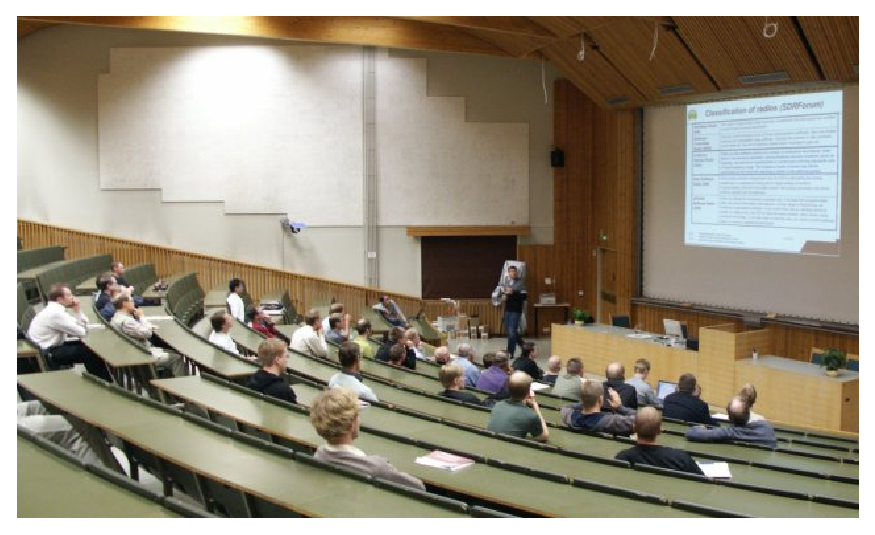
\includegraphics[height=8cm]{kuva2}
\end{center}
\caption{Kuvateksti, jossa on liitteen numerointi \label{liitekuva}}
\end{figure}
%%
Liitteiden taulukoiden numerointi on kuvien ja kaavojen kaltainen:
\begin{table}[htb]
\caption{Taulukon kuvateksti. \label{liitetaulukko}}
\begin{center}
\fbox{
\begin{tabular}{lp{0.5\linewidth}}
9.00--9.55  & Käytettävyystestauksen tiedotustilaisuus (osanottajat
ovat saaneet sähköpostitse valmistautumistehtävät, joten tiedotustilaisuus
voidaan pitää lyhyenä).\\
9.55--10.00 & Testausalueelle siirtyminen
\end{tabular}}
\end{center}
\end{table}
Kaavojen numerointi muodostaa liitteissä oman kokonaisuutensa:
\begin{eqnarray}
T_{ik} &=& -p g_{ik} + w u_i u_k + \tau_{ik},  \label{liitekaava3} \\
n_i    &=& n u_i + v_i.                        \label{liitekaava4}
\end{eqnarray}

\end{document}
